\subsection{Software structure}
The control is implemented on a Xilinx Zybo board which is a controller consisting of a FPGA part and a dual-core ARM Cortex-A9 processor.

Low-level drivers are implemented in the logic to allow the modules to run in parallel. The field orientated control as well as the interface to a PC is implemented on the processor which gives the possibility to have a higher abstraction. 

An overview of the system can be seen on figure \ref{fig:embedded_overview}. In the top is the processing system (PS) with an Interrupt Service Routine (ISR) and the control loop. The control loop outputs its result into a piece of block RAM from where the programmable logic (PL) can access it. The processing system also manages the interface to the PC which is done through UART.

\begin{figure}[H]
	\centering
	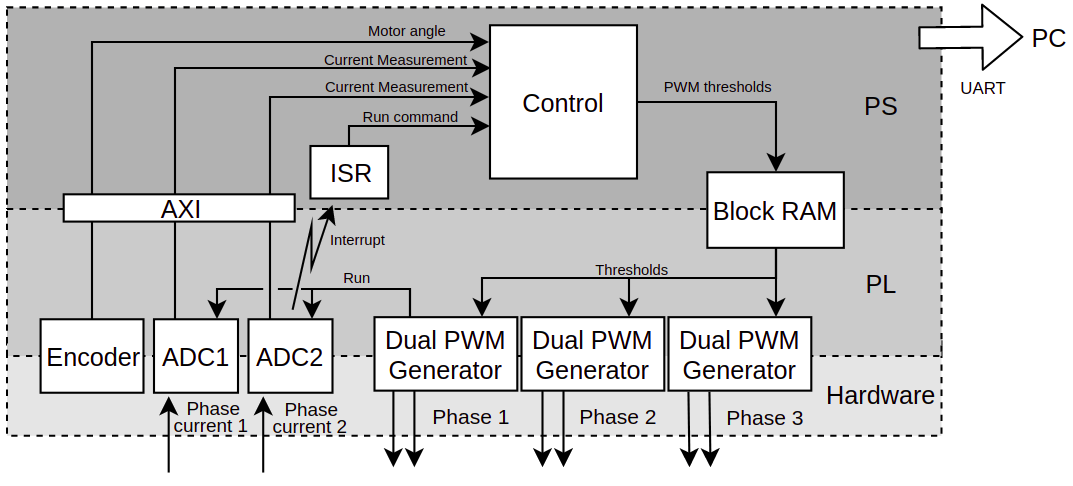
\includegraphics[width=1\linewidth]{pictures/software/embedded_overview.png}
	\caption{Embedded system overview}
	\label{fig:embedded_overview}
\end{figure}


In the programmable logic the drivers for three dual PWM generator are implemented. Each PWM generator control one phase in the inverter. The PWM generators all generate a pulse in the middle of their PWM periods. One of these are parsed to the ADC's and used to trigger a reading of the phase currents and the torque pedal. When the ADC's are done converting all inputs they produce an interrupt that triggers the ISR in the processing system.

The ADC readings as well as the encoder readings are parsed to the processing system through the AXI interface.



On figure \ref{fig:software_flow} the flowchart of the control loop implemented on the processing system can be seen. The system is waiting to receive the run command from the ISR which is triggered once every PWM period, see section \ref{sec:isr} for more about the ISR. 


\begin{figure}[H]
	\centering
	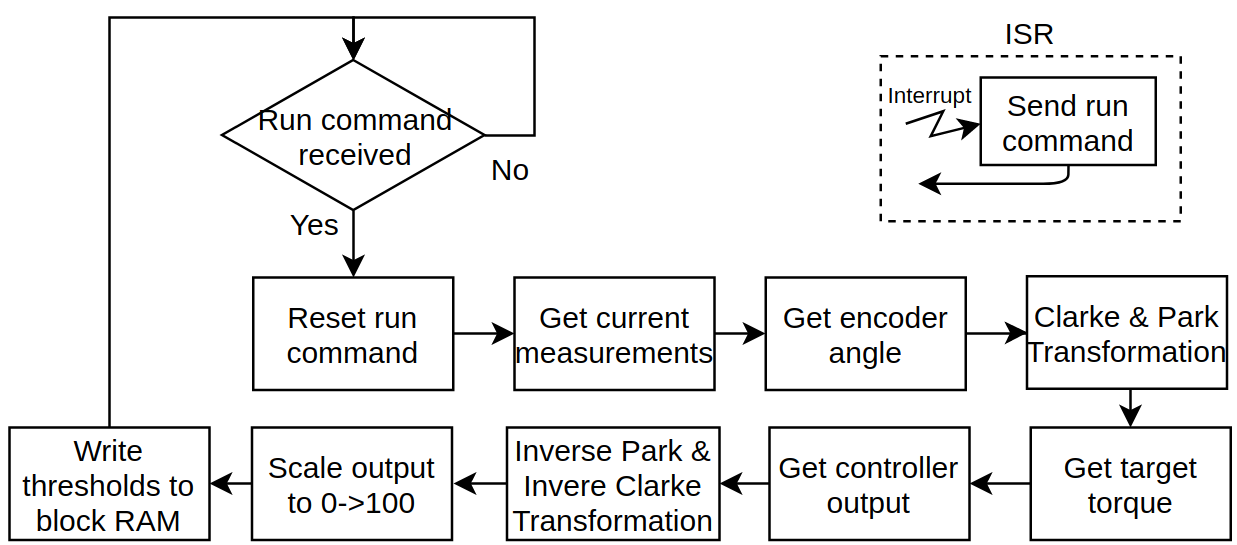
\includegraphics[width=0.9\linewidth]{pictures/software/software_flow.png}
	\caption{Processing System Overview}
	\label{fig:software_flow}
\end{figure}

When the run command is received it is first reset to get ready for the next command. Then the current measurements from the two ADC's are read into the system as well as the rotor angle from the encoder. A Clarke and a Park transformation is performed. The torque pedal position is read and the two PI controllers as discussed in section \ref{sec:control_system} perform the control. The result from the controllers are then transformed with an Inverse Park and an Inverse Clarke Transformation which produces three control signals. These signals are then linearly mapped to the range $0 \rightarrow 100$, which is what the PWM generators are compatible with. 
The thresholds are then written to a piece of block RAM shared between the PS and the PL. The PS will then wait for the next run command.



